\documentclass[11pt,aspectratio=169]{beamer}


\usetheme{lastig}

\colorlet{titlefgcolor}{LASTIGBlue}
\colorlet{accentcolor}{LASTIGRed}



\usepackage{mathptmx,amsmath,amssymb,graphicx,bibentry,bbm,babel,ragged2e}

\makeatletter

\newcommand{\noun}[1]{\textsc{#1}}
\newcommand{\jitem}[1]{\item \begin{justify} #1 \end{justify} \vfill{}}
\newcommand{\sframe}[2]{\frame{\frametitle{#1} #2}}

\newenvironment{centercolumns}{\begin{columns}[c]}{\end{columns}}
%\newenvironment{jitem}{\begin{justify}\begin{itemize}}{\end{itemize}\end{justify}}


\@ifundefined{showcaptionsetup}{}{%
 \PassOptionsToPackage{caption=false}{subfig}}
\usepackage{subfig}

\usepackage[utf8]{inputenc}
\usepackage[T1]{fontenc}



\makeatother


\begin{document}




\title[An empirical analysis of fuel prices in the US]{An empirical analysis of the spatial variability of fuel prices in the United States}
\date[17/02/2026]{\medskip S{\'e}minaire INSEE - DEE, 17/02/2026}
\author[Raimbault and Bergeaud]{Juste Raimbault$^{1}$ and Antonin Bergeaud$^{2}$\\
$^{1}$LaSTIG, Univ. Gustave Eiffel, IGN-ENSG\\
$^{2}$HEC Paris\smallskip\\
\texttt{juste.raimbault@ign.fr}}



\titleframe



%%%%%%%%%%%%%%%%%
\section{Introduction}
%%%%%%%%%%%%%%%%%



\sframe{Accidental fieldwork on the variability of gas prices}{

\begin{columns}
\begin{column}{0.21\textwidth}
\includegraphics[width=\textwidth]{../../Communication/figures/pic_sfi}\\
\includegraphics[width=\textwidth]{../../Communication/figures/pic_dunes}\\
\includegraphics[width=\textwidth]{../../Communication/figures/pic_grdteton}
\end{column}
\begin{column}{0.55\textwidth}
\includegraphics[width=\textwidth]{../../Communication/figures/roadtrip}
\end{column}
\begin{column}{0.21\textwidth}
\includegraphics[width=\textwidth]{../../Communication/figures/pic_rockies}\\
\includegraphics[width=\textwidth]{../../Communication/figures/pic_sf}\\
\includegraphics[width=\textwidth]{../../Communication/figures/pic_yosemite}
\end{column}
\end{columns}


%$\rightarrow$ In the US you fuel your (necessary big) car everywhere and everyday, and directly feel the strong variability of prices !

}



\sframe{Some questions in the fuel price litterature}{

\textbf{1. Spatial Dynamics and Behavioral Response}
    \begin{itemize}
        \item \textbf{Cross-border Arbitrage:} How do price discontinuities (e.g., AZ-CA border) drive ``fuel tourism'' and spatial tax competition? \cite{rietveld2001spatial}
        \item \textbf{Inter-modality:} How does spatial price heterogeneity shift user behavior between transportation modes? \cite{combes2005transport}
    \end{itemize}

    \textbf{2. Policy Design and Externalities}
    \begin{itemize}
        \item \textbf{Optimal Taxation:} How to design tax systems that internalize negative externalities (pollution, congestion) across diverse territories? \cite{gregg2009temporal}
        \item \textbf{Elasticity Heterogeneity:} How do consumption responses to price shocks vary by household income and geographic location? \cite{li2014gasoline}
    \end{itemize}

    \textbf{3. Price Transmission and Frictions}
    \begin{itemize}
        \item \textbf{Pass-through Dynamics:} What is the rate of transmission from crude oil to retail? \cite{gautier2015dynamics}
        \item \textbf{Asymmetric Adjustment:} Do pump prices react faster to wholesale increases than to decreases? \cite{deltas2008retail}
    \end{itemize}

}



\sframe{The geography of fuel prices}{

\textit{Spatio-temporal variability of Fuel Price can be linked to various aspects: geographical properties of a particular energy market, characteristics of the transportation system, interactions between transportation and territories.}

\justify

\textbf{Research Objective: } \textit{Empirical analysis of a large and detailed dataset of US fuel retail price, focusing on spatio-temporal variability}

\bigskip

$\rightarrow$ Focus on geographical patterns and structures

\medskip

$\rightarrow$ Complementarity of spatial analysis methods

\medskip

$\rightarrow$ Interdisciplinary point of view on a fundamentally heterogenous system

\bigskip

\textbf{Our contribution:}

\begin{itemize}
	\item 
\end{itemize}

}


%%%%%%%%%%%%%%%%%
\section{Dataset construction and visualisation}
%%%%%%%%%%%%%%%%%



\sframe{Dataset Construction}{

\justify

\textit{Crowdsourced Big Data as a new way to unveil structure of complex socio-technical systems}

\bigskip


$\rightarrow$ Construction of a large scale dataset covering most of US fuel stations on two months, by collecting crowdsourced data from the website \texttt{gasbuddy.com}

\bigskip

\textbf{Requirements for the crawler: } Flexibility, performance and anonymity

\medskip

\textbf{Architecture: } use open source tools developped by \cite{raimbault2019exploration}

\begin{itemize}
	\item pool of proxy tasks to pipe requests through \texttt{tor}
	\item manager monitors and launches collection tasks
	\item subtasks crawl and parse target webpages
\end{itemize}



}



\sframe{Dataset Summary}{

\begin{itemize}
\item $41\cdot 10^6$ unique observations, between January and March 2017\\$\rightarrow$ 5,204,398 gas station - day observations for main purchase mode and regular fuel, used in the analysis, aggregated at the county level
\item Socio-economic data from US Census Bureau and other official sources
\item Aggregation at the County level for the rest of the analysis
\end{itemize}


\bigskip

\begin{table}
\centering
\caption{Descriptive statistics on Fuel Price (\$ per gallon)}
\begin{tabular}{ccccccc}
\textbf{Mean} & \textbf{Std. Dev.} & \textbf{p10} & \textbf{p25} & \textbf{p50} & \textbf{p75} & \textbf{p90} \\
\hline
\cr
2.28 & 0.27 &  2.02  &  2.09  &  2.21  &  2.39  &  2.65  \\
\hline
\end{tabular}
\end{table}

}




\sframe{Data Exploration}{

\footnotesize

Interactive web-application for spatio-temporal exploration \cite{kwan2000interactive}

\url{https://analytics.huma-num.fr/geographie-cites/fuelprice/}

\centering

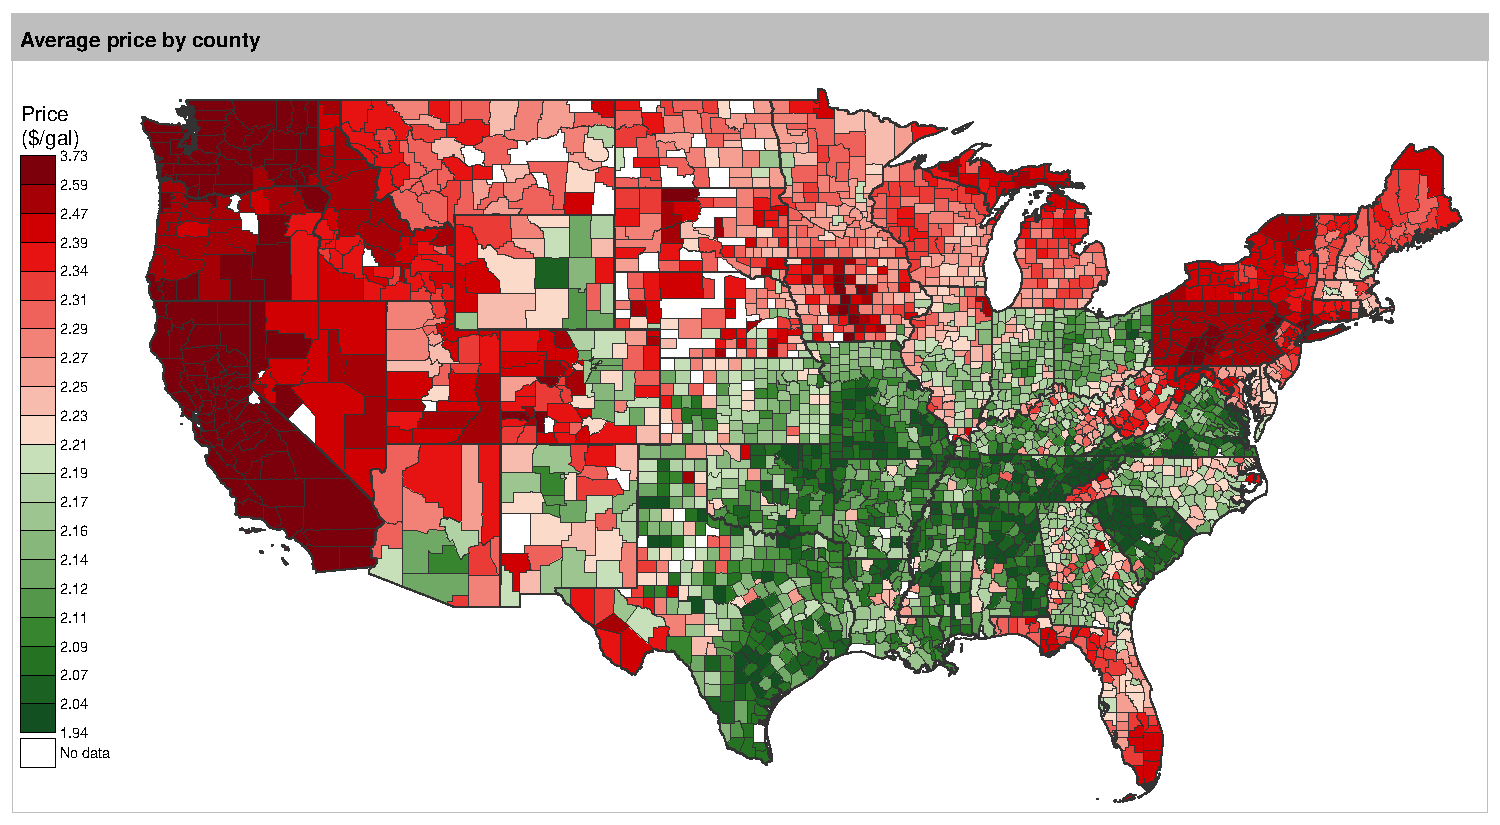
\includegraphics[width=0.8\textwidth]{../../Communication/figures/average_regular_map}

}




\section{Econometric analysis}


\sframe{Spatio-temporal correlations}{

\textit{Variability in space and time of Moran spatial auto-correlation index unveils strong non-stationnarity}

\bigskip

\includegraphics[width=0.45\textwidth,height=0.5\textheight]{../../Communication/figures/moran_days}
\includegraphics[width=0.45\textwidth,height=0.5\textheight]{../../Communication/figures/moran_decay_weeks}

}


\sframe{Geographically Weighted Regression}{

\justify


\begin{itemize}
\item \textbf{Geographically Weighted Regression} (GWR)~\cite{brunsdon1996geographically} to tackle spatial non-stationarity: capturing a spatially heterogeneous influence of socio-economic variable on prices
\item Models based on basic socio-economic variables: income, population, average wage,
jobs per capita, jobs
\item Multi-modeling using corrected AIC for model selection: find the best model and the best bandwidth controlling for overfitting
\end{itemize}

\bigskip
\bigskip

\textbf{Best model :}  $price = \beta\cdot\left( income, wage, percapjobs\right)$ with an optimal bandwidth around 75km (22 neighbors with adaptive bandwidth), interpreted as spatial stationarity scale of price processes in relation to economic agents.

}


\sframe{Geographically Weighted Regression: Results}{

\textit{Fitted coefficients and $R^2$ for the best model}

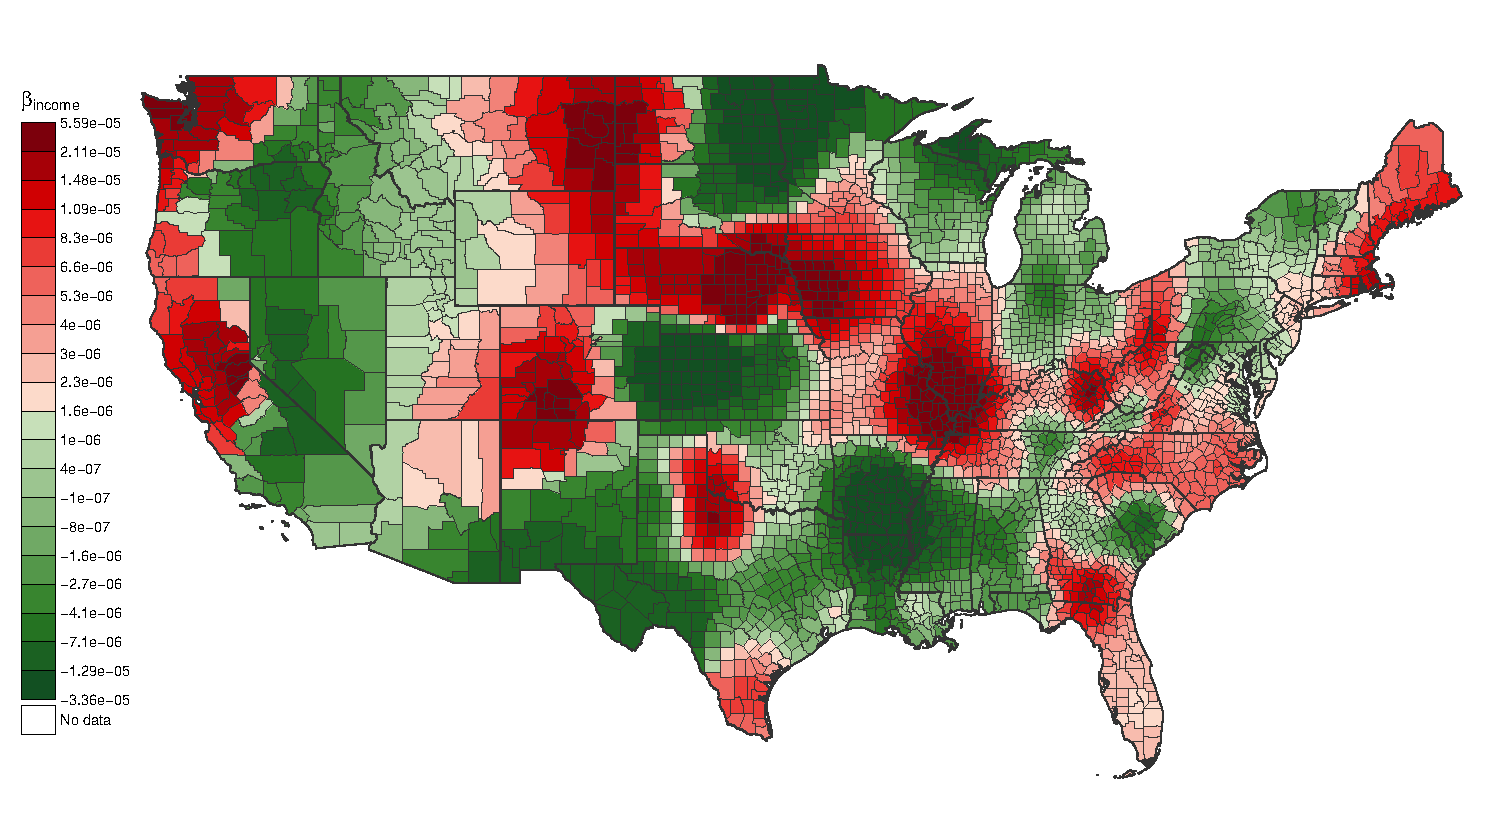
\includegraphics[width=0.45\textwidth,height=0.4\textheight]{../../Communication/figures/gwr_allbest_betaincome}
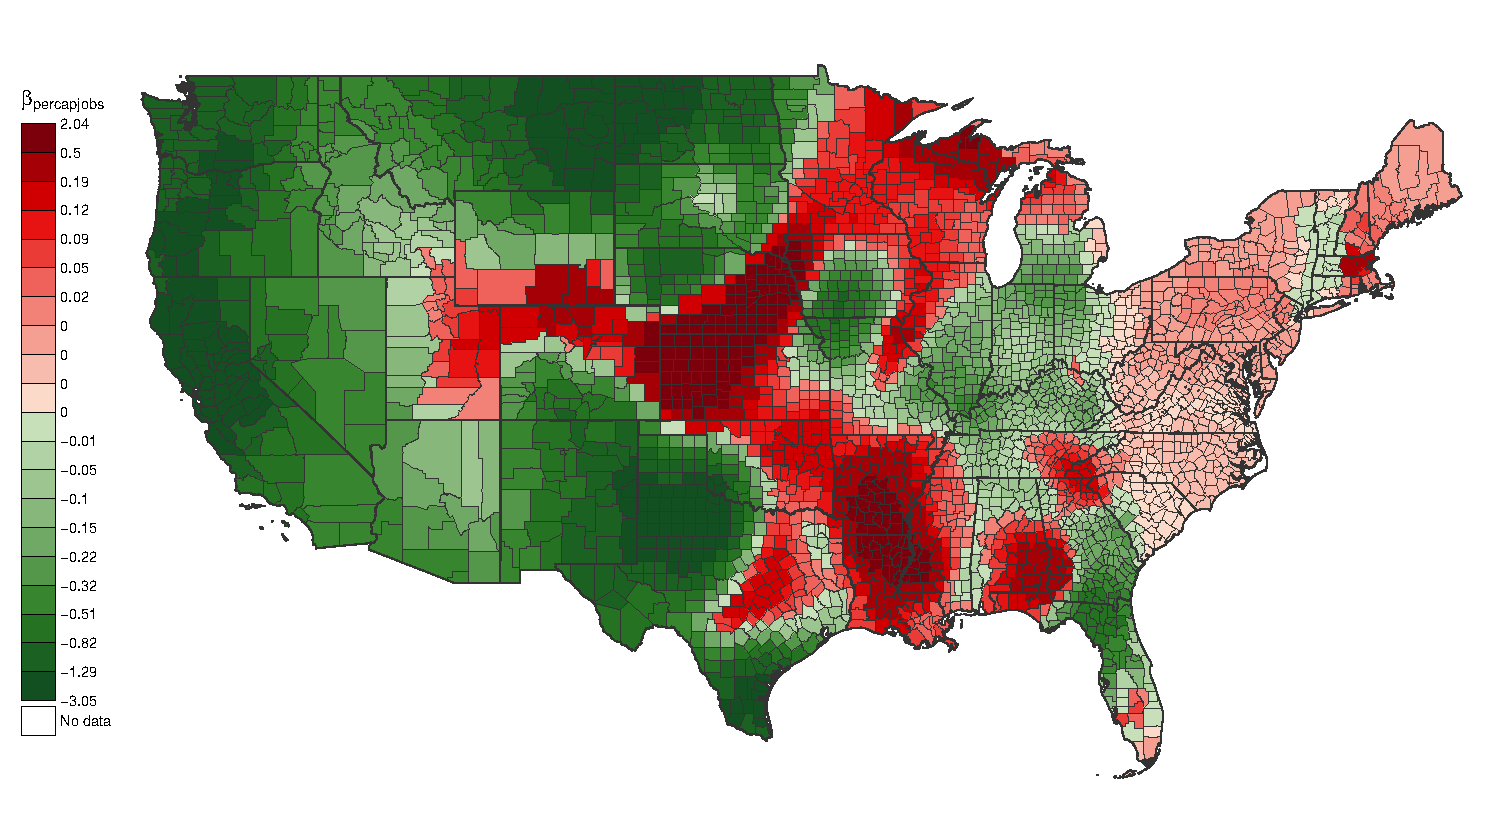
\includegraphics[width=0.45\textwidth,height=0.4\textheight]{../../Communication/figures/gwr_allbest_betapercapjobs}\\
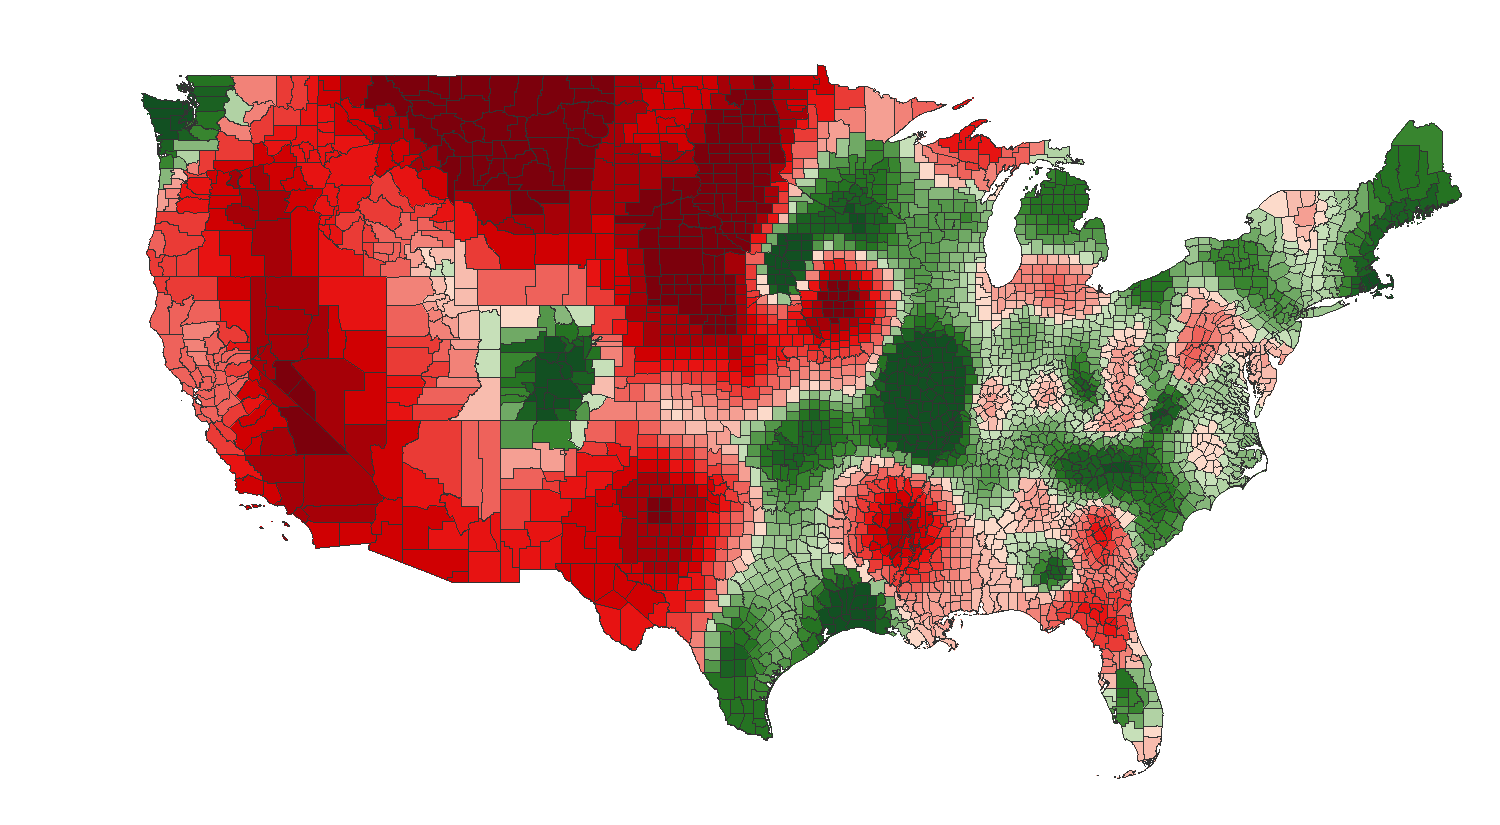
\includegraphics[width=0.45\textwidth,height=0.4\textheight]{../../Communication/figures/gwr_allbest_wage}
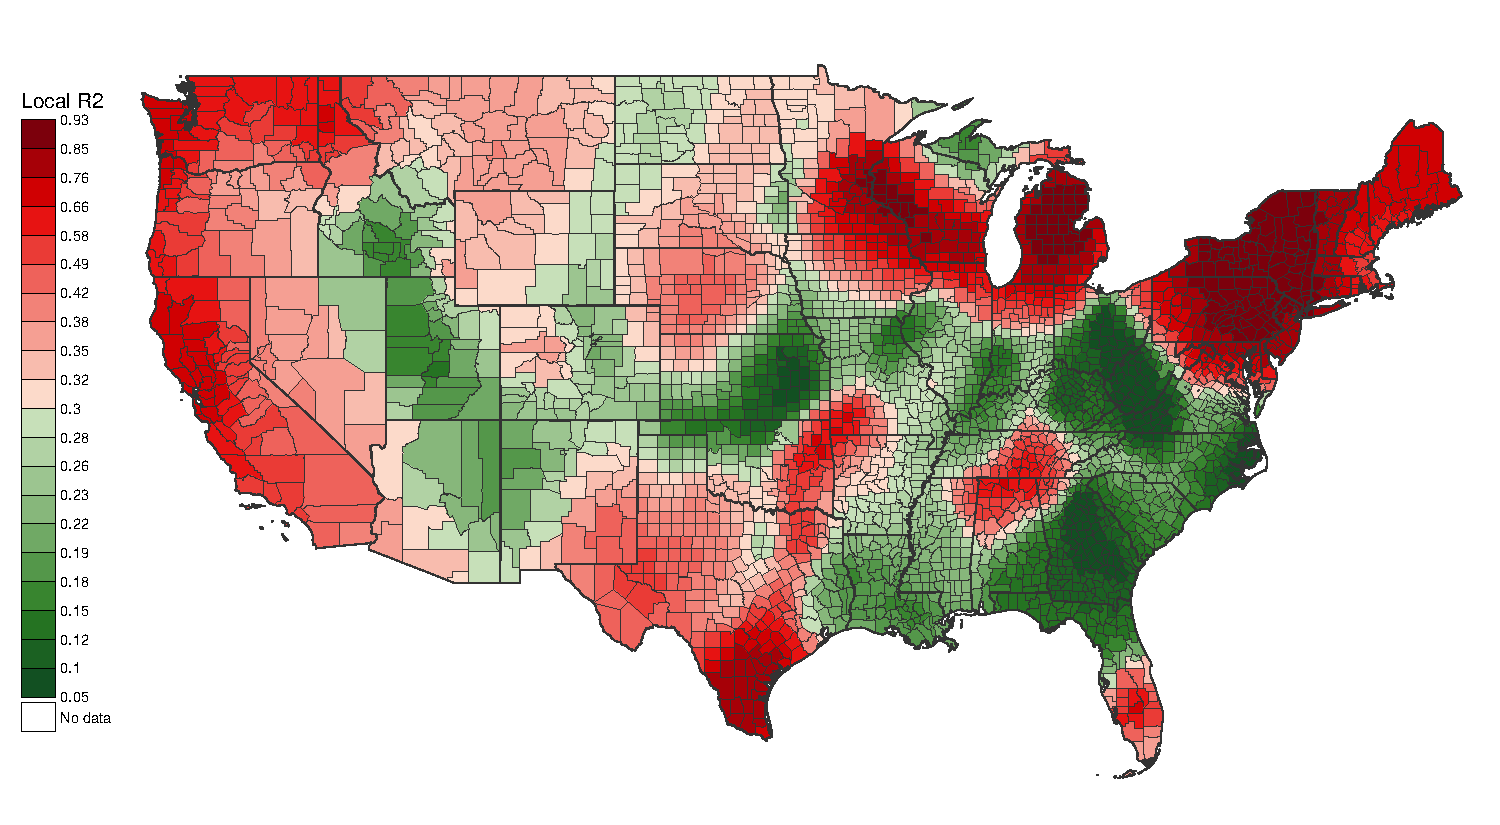
\includegraphics[width=0.45\textwidth,height=0.4\textheight]{../../Communication/figures/gwr_allbest_LocalR2}\\

}

\sframe{GWR summary}{

\textbf{1. Heterogeneous Spatial Performance}
    \begin{itemize}
        \item \textbf{Key Clusters:} High model fit on West Coast, South Border, North-East, and Chicago-Texas corridor.
        \item \textbf{Variable Regimes:} 
        \begin{itemize}
            \item \textit{Income:} Inverted influence based on coastal proximity (economic specialization).
            \item \textit{Wage/Employment:} Sharp East-West splits, suggesting cultural or structural drivers beyond state policy.
        \end{itemize}
    \end{itemize}

    \textbf{2. Spatial Stationarity Scale}
    \begin{itemize}
        \item \textbf{Optimal Bandwidth:} approximately log-normal distribution of distances with the adaptive optimal bandwidth
        \item Median distance of \textbf{77 km} (IQR: 30 km).
        \item \textbf{Possible interpretation:} defines the range of \textbf{coherent market competition} and the spatial stationarity of price-setting processes.
    \end{itemize}

}




\sframe{Multi-level Regression}{


Fixed effect regression at the level of the state : multi-level modeling to capture spatial effect of administrative boundaries

\begin{equation}
\label{eq:reg}
log(x_{i}) = \beta_0 + X_{i}\beta_1 + \beta_{s(i)} + \varepsilon_{i},
\end{equation}

\medskip

\begin{itemize}
\item Clustering of standard error at the state level motivated by the strong spatial autocorrelation: capture county-level variation controlling for State fixed effect
\item Regressing the log of price on a state fixed-effect explains 74\% of the variance
\item Influence of taxes: regressing the log of oil price on the level of state tax gives a R-squared of 0.33\%
\end{itemize}

}

\sframe{Multi-level Regression: results}{

\centering

\includegraphics[width=\linewidth]{figures/regression.png}


}



\sframe{Multi-level regression summary}{

\begin{itemize}
\item Strong influence of state-level tax
\medskip
\item Prices negatively correlated with population density 
\medskip
\item Fuel price also decreases with poverty
\medskip
\item It decreases with the extent to which a county has voted for a Republican candidate: suggests a circular link
\medskip
\item Overall, local socio-economic features have explanatory power even when removing State fixed effect
\end{itemize}


}




\section{Theoretical model}


\sframe{A minimal theoretical model}{

\textit{Modelling the role of population density in a minimal theoretical model:}

\medskip

\begin{itemize}
	\item Extension of the Salop model of spatial competition \cite{salop1977bargains}
	\item Exogenous population density
	\item Transportation cost is a function of the firms' output (gas stations)
\end{itemize}

}

\sframe{Model description}{

\footnotesize

\begin{itemize}
	\item N consumers $n=\{1..N\}$ and J gas station $j=\{1..J\}$, on a unit circle (positions $\theta(n)$ and  $\phi(j) = \frac{2\pi j }{J}$)
	\item Fixed population distribution $\mathcal{H}(\theta)$
	\item Price $p(j)$ gives a cost $C(n,j) = \eta p(j) \left|\theta(n)-\phi(j) \right|$ ($\eta$ consumption rate)
	
	\item Indifference condition between stations $j$ and $j+1$:

$$
p(j)\left(1+\eta\left(\theta(n)  -  \frac{2\pi j }{J}\right)\right) = p(j+1)\left(1-\eta\left(\theta(n)  -  \frac{2\pi (j+1) }{J}\right)\right)
$$

	\item Position of the indifferent customer:
$$
\theta(n) = \frac{1}{\eta}\frac{p(j+1)-p(j)}{p(j+1)+p(j)} + \frac{2\pi j}{J}+\frac{2\pi}{J}\frac{p(j+1)}{p(j+1)+p(j)} \equiv \theta(j, j+1)
$$


	\item Profit of gas station $j$:

$$
\pi(j, p(j), p(j+1), p(j-1)) = \left(p(j)-P\right) \int_{\theta(j-1, j)}^{\theta(j, j+1)}{ d\mathcal{H}(\theta)}
$$

\end{itemize}

}

\sframe{Model resolution}{

Maximisation of $\pi$ for each station gives the First Order Condition giving the prices $\vec{p}$:

\begin{equation}
\label{eq:tosolve}
\int_{\theta(j-1, j)}^{\theta(j, j+1)}{ d\mathcal{H}(\theta)} = \left(\frac{2}{\eta} +\frac{2\pi}{J}\right)(p(j)-P)\left(\frac{p(j+1)h(\theta(j,j+1))}{\left(p(j)+p(j+1)\right)^2} +  \frac{p(j-1)h(\theta(j-1,j))}{\left(p(j)+p(j-1)\right)^2}\right)
\end{equation}

\bigskip

\begin{itemize}
	\item No tractable solution for any distribution $\mathcal{H}$
	\item Minimise computationally $C\left[h,J,\eta,P\right] = \sum_j f_j(\vec{p},h,J,\eta,P)^2$ with a genetic algorithm 
\end{itemize}

}


\sframe{Computational resolution of the minimal model}{


\includegraphics[width=0.3\linewidth]{../../Paper/figures/fig7a.png}
\includegraphics[width=0.3\linewidth]{../../Paper/figures/fig7b.png}
\includegraphics[width=0.3\linewidth]{../../Paper/figures/fig7c.png}


}





%%%%%%%%%%%%%%%%%
\section{Discussion}
%%%%%%%%%%%%%%%%%


\sframe{Discussion}{

$\rightarrow$ Complementarity of Spatial analysis and econometrics methods


$\rightarrow$ Possible design of territory-targeted car-regulation policies, allowing both sustainability and territorial equity

\medskip

\textbf{Future work:}

$\rightarrow$ Microscopic data analysis (requires precise geocoding), calibration of consumer/producer behavior models


$\rightarrow$ Longer time series and time-series modeling


$\rightarrow$ Parametrization of a large-scale ABM of the spatialized fuel market: investigation of  adaptive policies effects at the local and global level


$\rightarrow$ Similar analysis on French open data


}




\sframe{Conclusion}{

$\rightarrow$ A novel insight into spatio-temporal dynamics of fuel price and their determinants thanks to big data harvesting

\medskip

$\rightarrow$ Complementary approaches and conclusions through GWR and multi-level modeling

\medskip

$\rightarrow$ Fundamental role of spatio-temporal non-stationarity and existence of typical stationarity scales


\bigskip
\bigskip
\bigskip

All code and aggregated data available at \texttt{https://github.com/JusteRaimbault/EnergyPrice}


}






%%%%%%%%%%%%%%%%%%%%%
\begin{frame}[allowframebreaks]
\frametitle{References}
\bibliographystyle{apalike}
\bibliography{biblio}
\end{frame}
%%%%%%%%%%%%%%%%%%%%%%%%%%%%





%%%%%%
\sframe{Spatial Heterogeneity}{

Spatial Autocorrelation as an index of spatial variability, for link $i$

\begin{equation}
\rho_i = \frac{1}{K}\cdot \sum_{i\neq j}{w_{ij}\cdot (c_i - \bar{c})(c_j - \bar{c})}
\end{equation}

with spatial weights  $w_{ij} = \exp{\left(\frac{-d_{ij}}{d_0}\right)}$

}



%%%%%%
\sframe{GWR Residuals}{

\centering

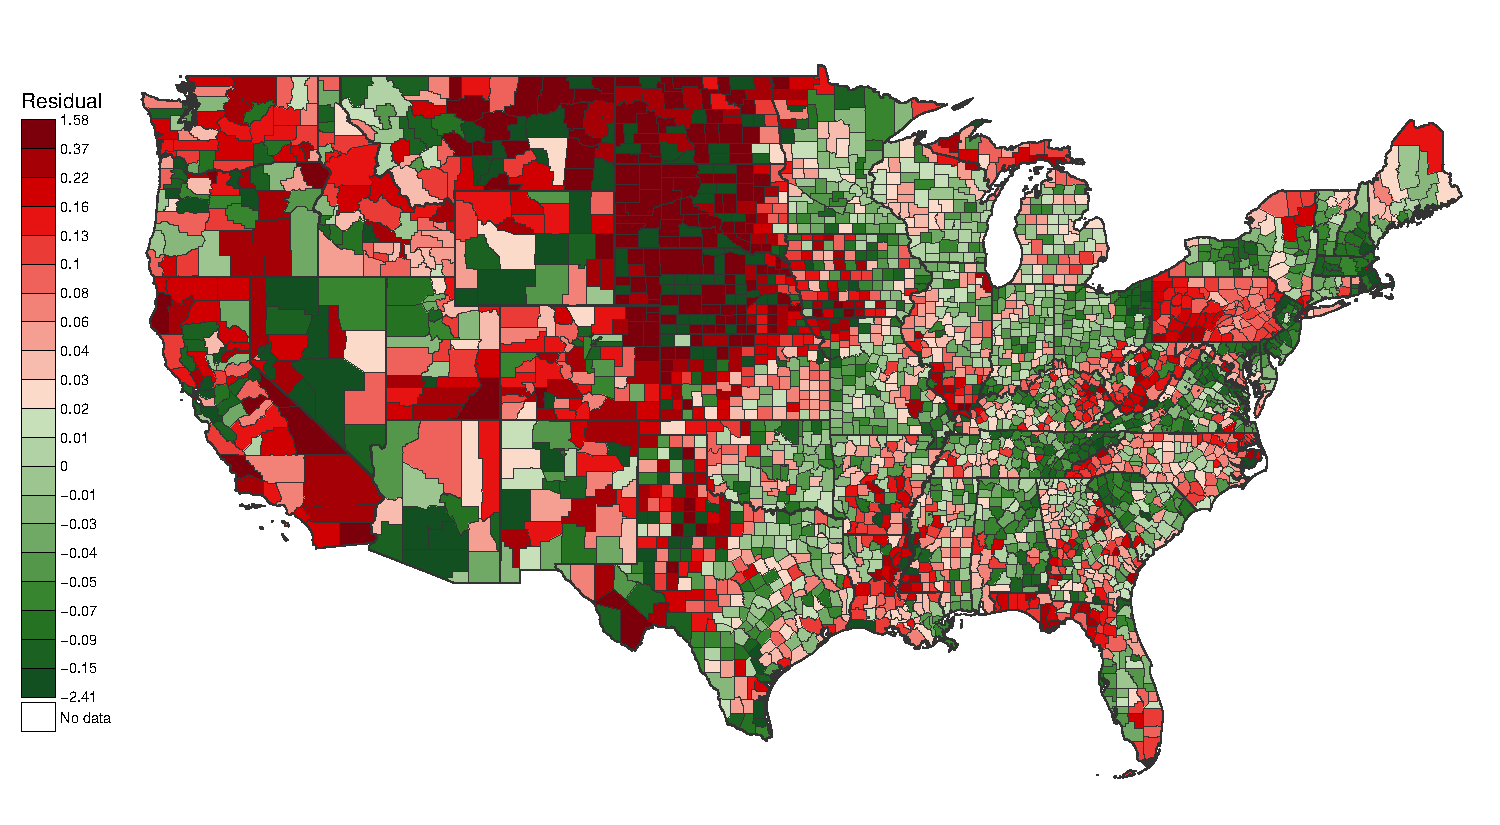
\includegraphics[width=\textwidth]{../../Communication/figures/gwr_allbest_residual}

}


\sframe{Socio-economic variables}{

\begin{table}[]
    \centering
    \caption{Source and description of the county level variables}
    \label{tab:county_var_desc}
    \begin{tabular}{lp{7cm}l}
    \hline
    Variable     &  Description & Source \\
    \cmidrule(r){1-1}
     \cmidrule(r){2-2}
      \cmidrule(r){3-3}
    \cr
    Density     &  Household units per sq miles & Census 2010 \\
    Unemployment & Total employed over labor force in 2017 & BLS \\
    Nb Stations & Number of gas station & Own calculation \\
    Manuf & Employment share of the manufacturing sector in 2016 & CBP - Census \\
    Bachelor & Share of population over 25 with a bachelor degree in 2017 & ACS \\
    Cars & Share of people over 16 using their car to commute in 2017 & ACS \\
    Poverty & Share of people considered in poverty by SAIPE program & SAIPE - Census \\
    Vote GOP & Share of voters that voted for a republican candidate in the general elections from 2000 & MIT election lab \\
    \hline
    \end{tabular}
\end{table}

}


\sframe{Socio-economic variables}{

\begin{table}[]
    \centering
    \caption{Descriptive statistics}
    \label{tab:county_var_stat_desc}
    \begin{tabular}{l ccccccc l}
    \hline
    Variable     &  mean & sd & p10 & p25 & p50 & p75 & p90 & units\\
    \cmidrule(r){1-1}
    \cmidrule(r){2-8}
    \cmidrule(r){9-9}

    \cr
    Density     &  113.4 & 823.8 & 2.2 & 8.4 & 21.0 & 51.5 & 164.2 & Households per sq mile\\
    Unemployment (x100)& 4.6 & 1.6 & 2.9 & 3.5&4.3 & 5.3 & 6.5 & Share\\
    Nb Stations & 28.0&65.9&1.7&3.3&9.4&24.7&64.9& Number \\
    Manuf (x100) & 19.3&17.0&0&6.1&15.4&28.5&43.0& Share \\
    Bachelor (x100) & 21.2&9.3&12.1&14.7&19&25.3&33.7&Share \\
    Cars (x100) & 89.5&7.3&82.5&87.8&91.3&93.5&95 &Share\\
    Poverty (x100) & 15.4 & 6.2 & 8.7&10.9&14.4&18.4&23.4 &Share \\
    Vote GOP (x100) & 59.4&13.2&41.8&51.4&60.5&68.7&75.5& Share\\
    \hline
    \end{tabular}
\end{table}

}





%%%%%%
\sframe{High dimensional fixed effects}{

With $x_{i,s,c,t}$ the fuel price in day $t$, in gas station $i$, in state $s$ and in county $c$, we start by running high dimensional fixed effect regressions

\begin{eqnarray}
x_{i,s,c,t} &=& \beta_s + \varepsilon_{i,s,c,t} \\
x_{i,s,c,t} &=& \beta_c + \varepsilon_{i,s,c,t} \\
x_{i,s,c,t} &=& \beta_i + \varepsilon_{i,s,c,t}\\
\end{eqnarray}

Where $\varepsilon_{i,s,c,t}$ contains an idiosyncratic error and a day fixed effect.

$\rightarrow$ It confirms that most of the variance can be explained by a state fixed effect and that integrating more accurate levels has only small effect on the fit of our model as measured by the R-squared.


}


\end{document}







